\chapter{Material adicional}
\label{chap:adicional}

\lettrine{E}{ste} anexo recoge fragmentos de código e implementación que no
resultan imprescindibles para seguir el cuerpo principal de la memoria, pero
que ilustran con detalle dos decisiones técnicas mencionadas en los
capítulos~\ref{chap:diseno} y~\ref{chap:implementacion} —la detección de
solapamiento de reservas a nivel de base de datos y el algoritmo de
generación de emparejamientos de torneos— además de un recorrido guiado por
la gestión completa de un torneo.

\section{Migración V4 — Índice de solapamiento de reservas}
\label{sec:anexo_migracion_v4}

La detección de conflictos de horario (RF-14, sección~\ref{sec:requisitos_funcionales})
podría implementarse comprobando en memoria todas las reservas existentes de
una pista, pero esto no escala y, sobre todo, no es seguro frente a
condiciones de carrera entre peticiones concurrentes. La migración
\texttt{V4\_\_add\_booking\_overlap\_index.sql} añade un índice parcial que
permite delegar esa comprobación en PostgreSQL:

\begin{lstlisting}[language=SQL]
CREATE INDEX idx_bookings_field_time_status
    ON bookings (field_id, start_time, end_time)
    WHERE status IN (1, 2);
\end{lstlisting}

El índice es \textbf{parcial}: solo cubre las reservas en estado
\texttt{PENDING} (1) o \texttt{CONFIRMED} (2), que son las únicas relevantes
para el cálculo de solapamiento. Las reservas \texttt{CANCELLED} y
\texttt{COMPLETED} quedan fuera, lo que mantiene el índice pequeño y rápido
incluso a medida que crece el histórico de reservas del sistema. La consulta
de solapamiento (\texttt{BookingRepository.existsConflict}) se apoya
directamente en este índice para resolver en una sola consulta SQL si existe
ya una reserva activa que se solape con el rango horario solicitado.

\section{Algoritmo de generación de cuadros de torneo}
\label{sec:anexo_bracket_generator}

\texttt{BracketGeneratorService} es un servicio de dominio puro —sin
dependencias de persistencia ni de Spring más allá de la anotación
\texttt{@Service}— invocado por
\texttt{Close\-Registration\-And\-Generate\-Bracket\-Use\-Case} al cerrar la inscripción
de un torneo. Selecciona el algoritmo según el formato de competición:

\begin{lstlisting}[language=Java]
public List<Match> generate(
        Tournament tournament, List<TournamentPair> confirmedPairs) {
    return switch (tournament.format()) {
        case ROUND_ROBIN ->
            generateRoundRobin(tournament, confirmedPairs);
        case ELIMINATION ->
            generateElimination(tournament, confirmedPairs);
        case GROUPS_AND_ELIMINATION ->
            generateGroupsAndElimination(tournament, confirmedPairs);
    };
}
\end{lstlisting}

Para el formato \texttt{ROUND\_ROBIN} se genera un partido por cada pareja de
parejas distintas (todos contra todos):

\begin{lstlisting}[language=Java]
private List<Match> generateRoundRobin(
        Tournament t, List<TournamentPair> pairs) {
    var matches = new ArrayList<Match>();
    for (int i = 0; i < pairs.size(); i++) {
        for (int j = i + 1; j < pairs.size(); j++) {
            var a = pairs.get(i).pairId();
            var b = pairs.get(j).pairId();
            matches.add(buildMatch(t.tournamentId(), a, b, 1, null));
        }
    }
    return matches;
}
\end{lstlisting}

Para el formato \texttt{ELIMINATION}, las parejas se mezclan aleatoriamente y
se emparejan para la primera ronda; las rondas siguientes se crean como
partidos \textit{placeholder} sin parejas asignadas (\texttt{pairAId} y
\texttt{pairBId} a \texttt{null}), que se completan progresivamente a medida
que se conocen los ganadores de la ronda anterior:

\begin{lstlisting}[language=Java]
private List<Match> generateElimination(
        Tournament t, List<TournamentPair> pairs) {
    var shuffled = new ArrayList<>(pairs);
    Collections.shuffle(shuffled);

    var matches = new ArrayList<Match>();
    int n = shuffled.size();

    // Ronda 1: parejas reales
    for (int i = 0; i < n; i += 2) {
        var a = shuffled.get(i).pairId();
        var b = shuffled.get(i + 1).pairId();
        matches.add(buildMatch(t.tournamentId(), a, b, 1, null));
    }

    // Rondas siguientes: placeholders, se rellenan
    // al completarse la ronda anterior
    int round = 2;
    int matchesInRound = n / 4;
    while (matchesInRound >= 1) {
        for (int i = 0; i < matchesInRound; i++) {
            matches.add(
                buildMatch(t.tournamentId(), null, null, round, null));
        }
        round++;
        matchesInRound /= 2;
    }
    return matches;
}
\end{lstlisting}

Esta estrategia de \textit{placeholders} evita tener que regenerar la
estructura completa del cuadro cuando se reporta el resultado de un partido:
\texttt{Close\-Registration\-And\-Generate\-Bracket\-Use\-Case} solo necesita localizar el
partido de la ronda siguiente correspondiente y rellenar el hueco vacante con
el identificador del ganador.

El formato \texttt{GROUPS\_AND\_ELIMINATION} combina ambas estrategias:
reparte las parejas en grupos de cuatro y aplica \textit{round robin} dentro
de cada grupo, seguido de una fase eliminatoria con \textit{placeholders} para
los dos primeros clasificados de cada grupo.

\section{Caso de uso guiado: gestión completa de un torneo}
\label{sec:anexo_gestion_torneo}

Esta sección recorre, mediante capturas reales de la aplicación, el ciclo de
vida completo de un torneo en formato \texttt{ROUND\_ROBIN}: su creación por
parte de un administrador, la inscripción de las parejas participantes y el
desarrollo del torneo hasta obtener la clasificación final. El detalle
funcional de cada paso —los requisitos que satisface y las reglas de negocio
que aplica— se describe en las secciones~\ref{sec:requisitos_funcionales}
y~\ref{sec:ciclo_torneo}; aquí se documenta únicamente el recorrido de
principio a fin sobre la interfaz.

\subsection{Creación del torneo}

Desde el panel de administración, el administrador crea un torneo indicando
el centro, el nombre, el formato de competición (\texttt{ROUND\_ROBIN} en
este caso), el número máximo de parejas y las fechas de inicio y fin
(figura~\ref{fig:anexo_torneo_creacion}). Al confirmarse, el torneo queda
registrado en estado \texttt{DRAFT} (figura~\ref{fig:anexo_torneo_creado}),
sin ser todavía visible para las inscripciones.

\begin{figure}[ht]
\centering
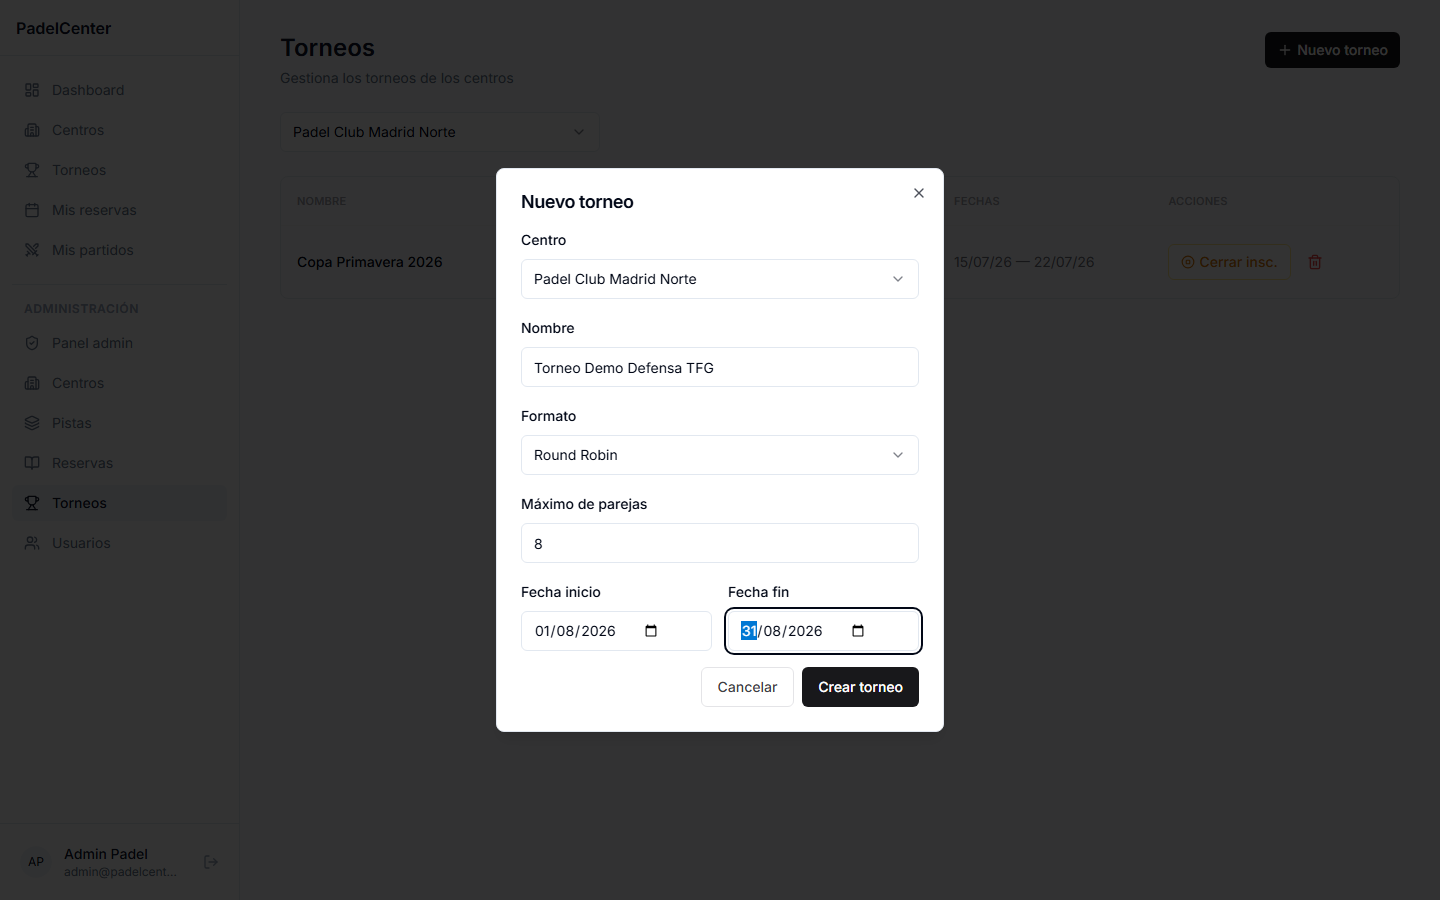
\includegraphics[width=0.7\textwidth]{imaxes/torneo-demo/d06-nuevo-torneo-relleno.png}
\caption{Formulario de creación de un torneo, con formato Round Robin y 8 parejas máximo.}
\label{fig:anexo_torneo_creacion}
\end{figure}

\begin{figure}[ht]
\centering
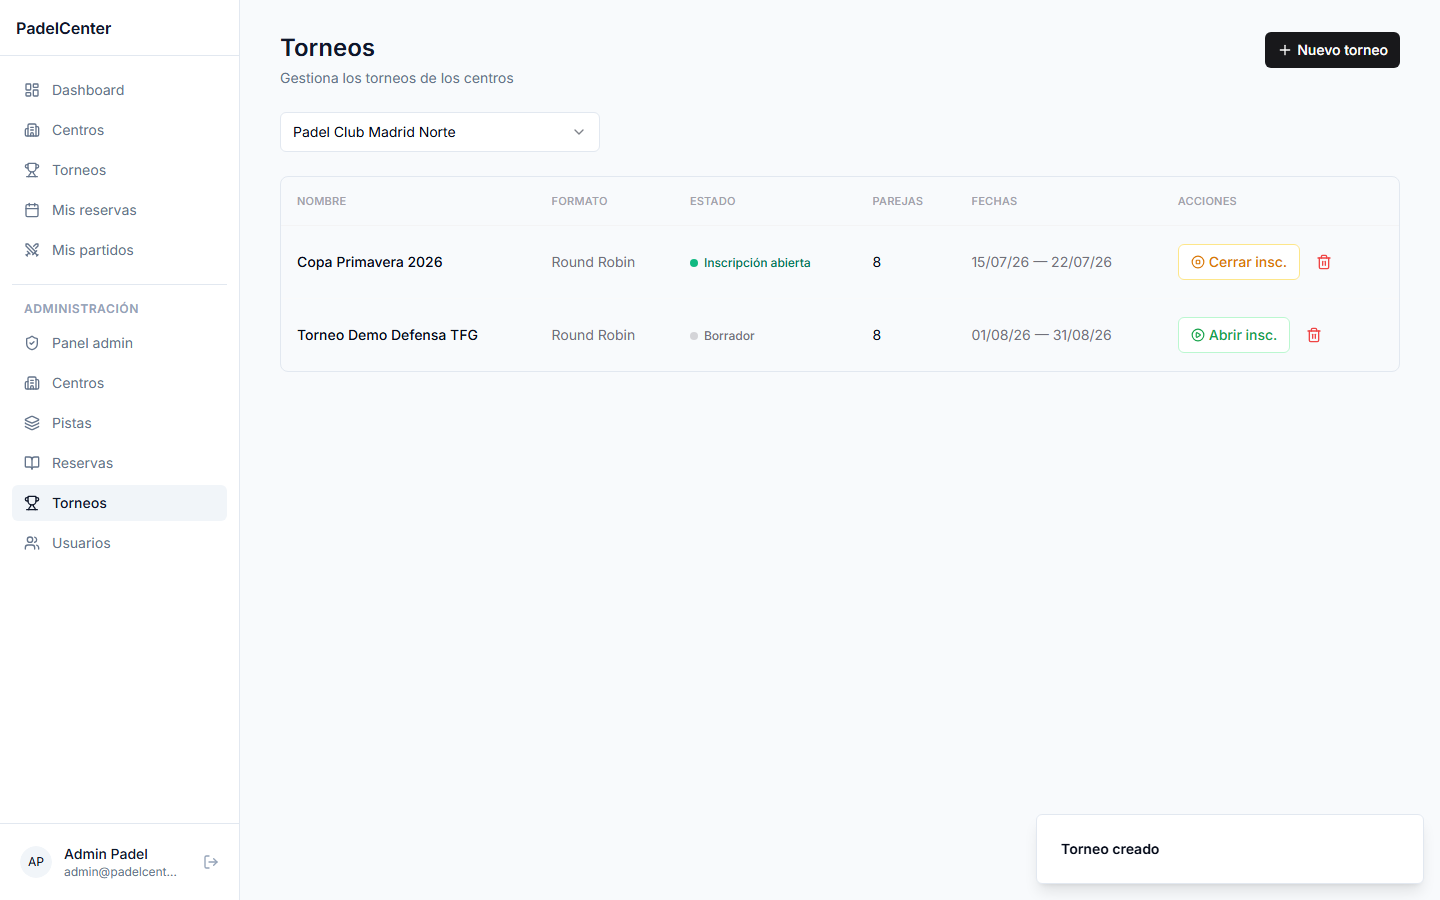
\includegraphics[width=0.7\textwidth]{imaxes/torneo-demo/d07-torneo-creado.png}
\caption{Torneo creado en estado \texttt{DRAFT}, pendiente de abrir inscripción.}
\label{fig:anexo_torneo_creado}
\end{figure}

Una vez creado, el administrador abre el período de inscripción
(figura~\ref{fig:anexo_torneo_inscripcion_abierta}), momento en el que el
torneo pasa a estado \texttt{REGISTRATION\_OPEN} y los jugadores ya pueden
apuntarse.

\begin{figure}[ht]
\centering
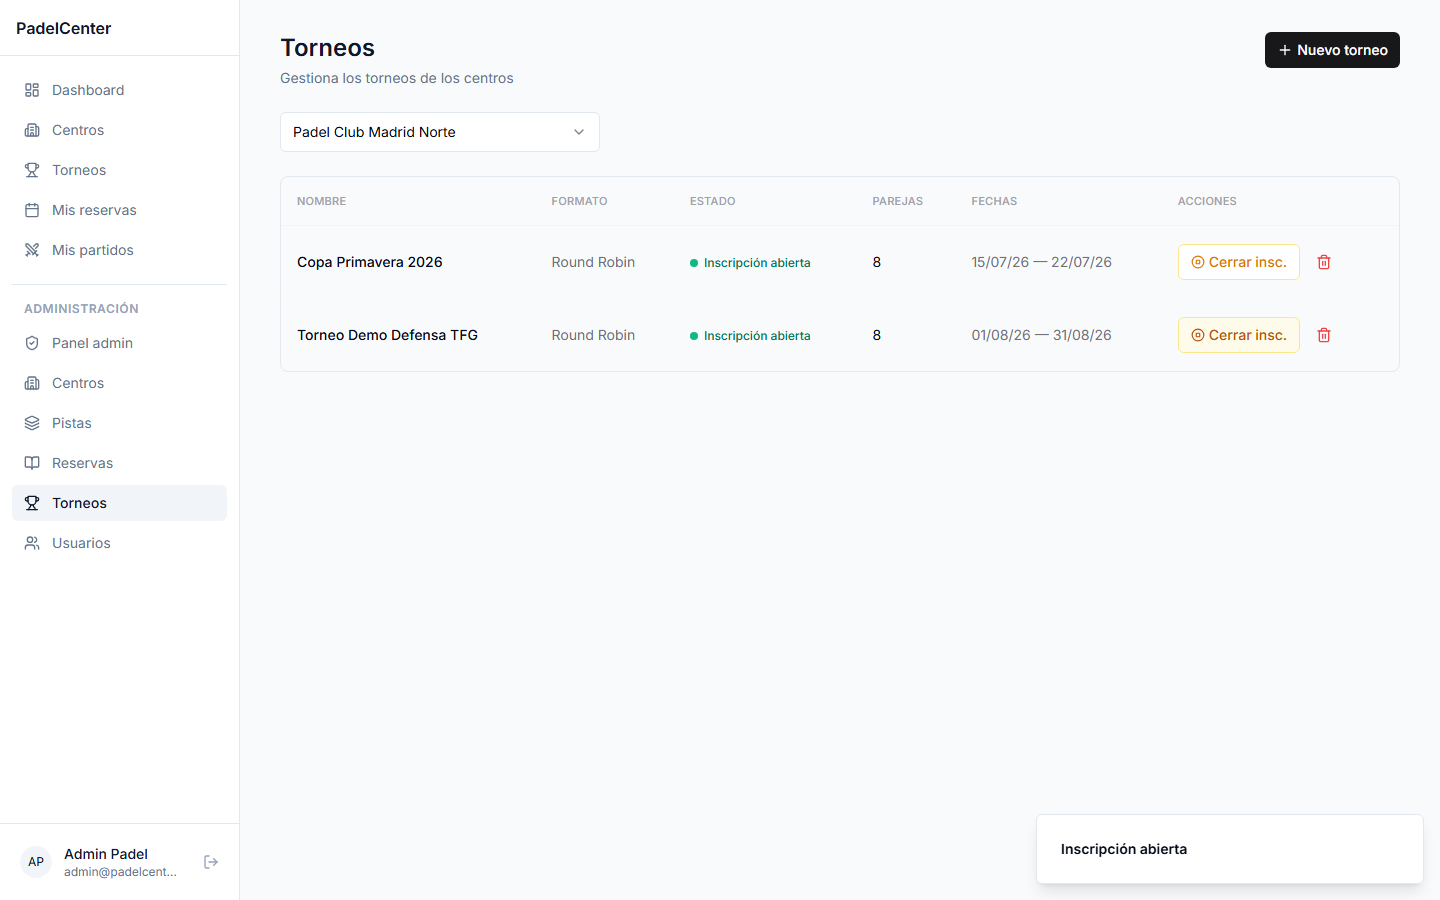
\includegraphics[width=0.7\textwidth]{imaxes/torneo-demo/d08-inscripcion-abierta.png}
\caption{Torneo con inscripción abierta, listo para recibir parejas.}
\label{fig:anexo_torneo_inscripcion_abierta}
\end{figure}

\subsection{Inscripción de parejas}

Con la inscripción abierta, un jugador se apunta al torneo formando pareja
con otro usuario. Al confirmarse la inscripción
(figura~\ref{fig:anexo_torneo_inscripcion_confirmada}), la pareja queda
registrada en estado \texttt{PENDING}, a la espera de que el segundo miembro
la confirme; este proceso se repite hasta completar las parejas necesarias
para cerrar la inscripción.

\begin{figure}[ht]
\centering
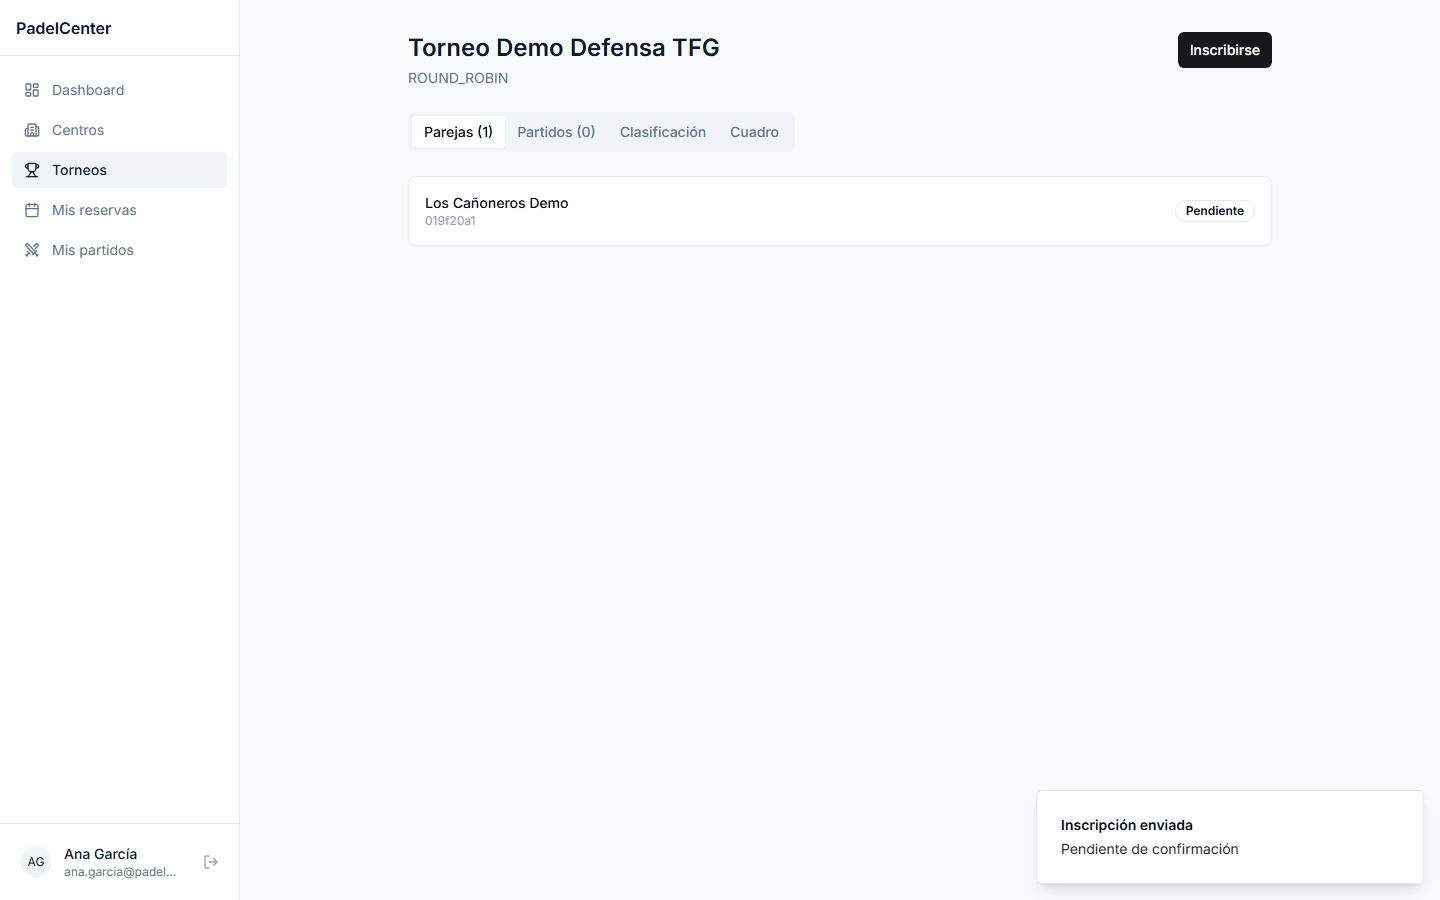
\includegraphics[width=0.7\textwidth]{imaxes/torneo-demo/d19-inscripcion-confirmada.png}
\caption{Inscripción de una pareja confirmada en el torneo.}
\label{fig:anexo_torneo_inscripcion_confirmada}
\end{figure}

\subsection{Desarrollo del torneo}

Con las cuatro parejas confirmadas, el administrador cierra la inscripción.
El sistema genera automáticamente, en una única operación atómica, los seis
partidos de la liguilla Round Robin entre todas las parejas
(figura~\ref{fig:anexo_torneo_partidos_generados}), y el torneo pasa a
estado \texttt{IN\_PROGRESS}.

\begin{figure}[ht]
\centering
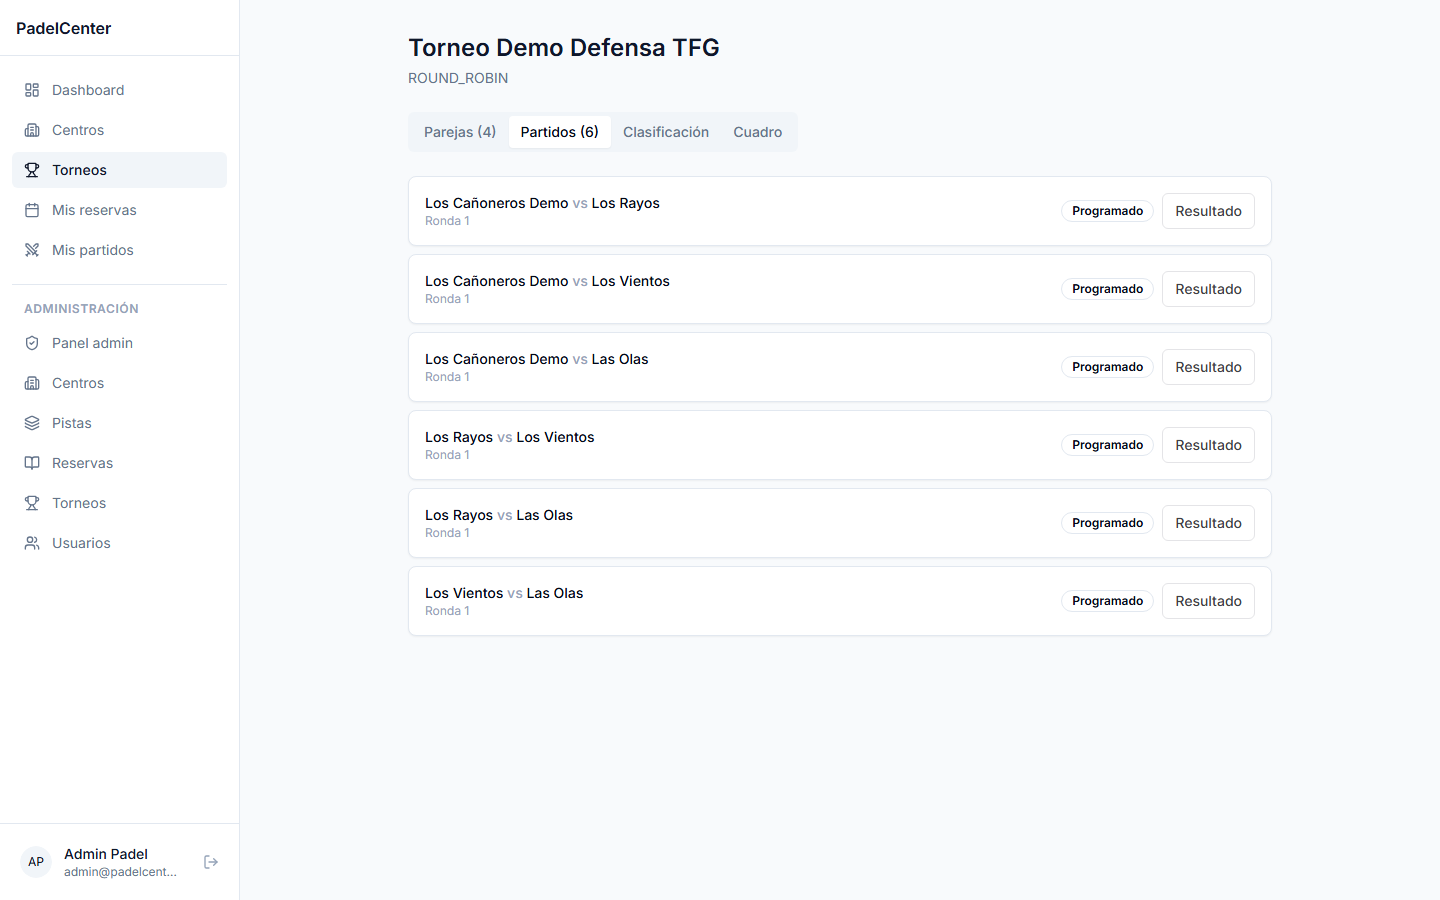
\includegraphics[width=0.7\textwidth]{imaxes/torneo-demo/d21-partidos-generados.png}
\caption{Partidos generados automáticamente al cerrar la inscripción.}
\label{fig:anexo_torneo_partidos_generados}
\end{figure}

A medida que se disputan los partidos, el administrador o el manager del
centro registran el resultado de cada uno —ganador y marcador—
(figura~\ref{fig:anexo_torneo_resultado}). Este paso se repite para los seis
partidos de la liguilla.

\begin{figure}[ht]
\centering
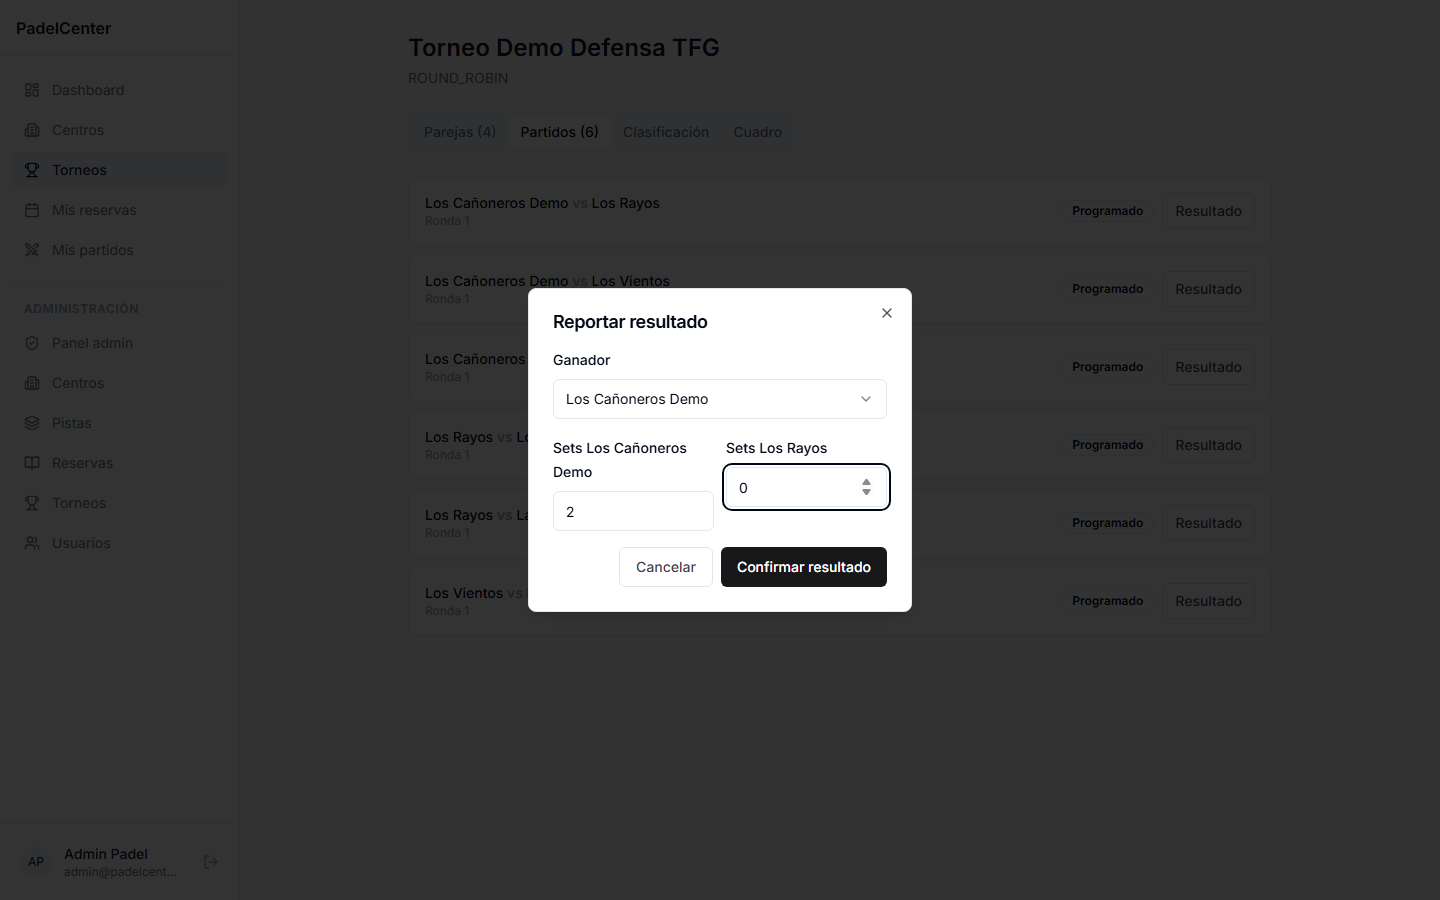
\includegraphics[width=0.7\textwidth]{imaxes/torneo-demo/d23-resultado-relleno.png}
\caption{Registro del resultado de un partido de la liguilla.}
\label{fig:anexo_torneo_resultado}
\end{figure}

Con todos los resultados registrados, el sistema calcula y expone la
clasificación final en tiempo real (figura~\ref{fig:anexo_torneo_clasificacion}),
determinada por el número de victorias y la diferencia de sets, dando por
completado el ciclo de vida del torneo.

\begin{figure}[ht]
\centering
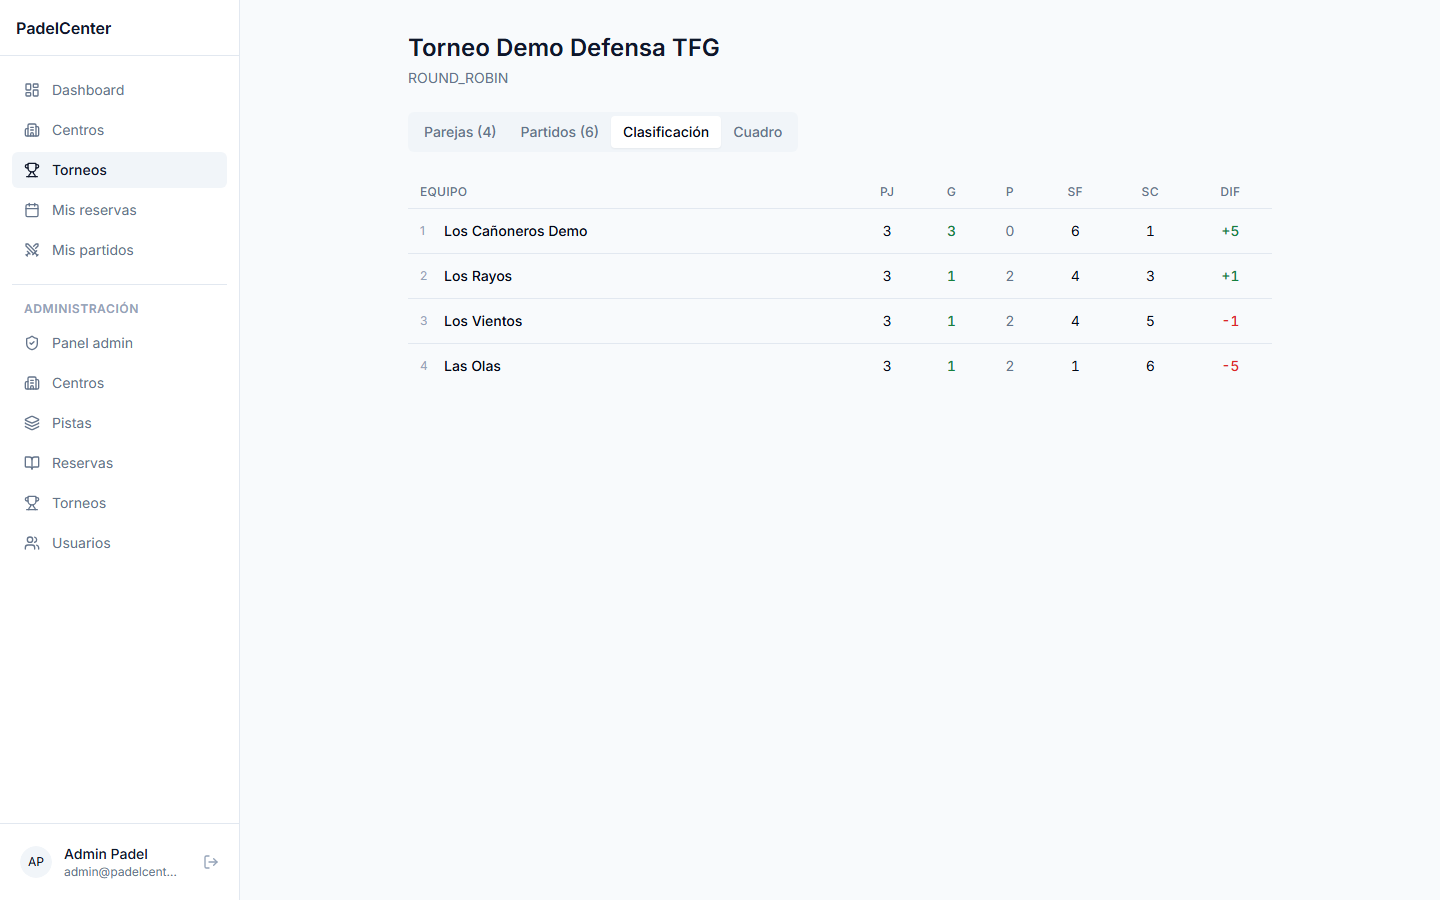
\includegraphics[width=0.7\textwidth]{imaxes/torneo-demo/d25-clasificacion.png}
\caption{Clasificación final de la liguilla Round Robin.}
\label{fig:anexo_torneo_clasificacion}
\end{figure}
